\newpage
\usecasebase{Eliminazione account}
\label{usecase:Eliminazione account}

\begin{figure}[h]
	\centering
	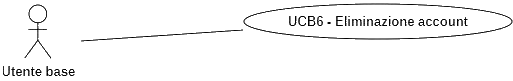
\includegraphics[width=0.8\textwidth]{./uml/UCB6.png} 
	\caption{Eliminazione account}
	\label{fig:UCB7}
  \end{figure}

\begin{itemize}
	\item \textbf{Attore principale:} Utente base.

	\item \textbf{Precondizioni:}
	      \begin{itemize}
		      \item L'Utente base ha eseguito correttamente l'accesso al Sistema come Utente base (vedi \autoref{usecase:Effettua accesso}).
		      \item L'Utente base si trova nella sua Area personale.
	      \end{itemize}

	\item \textbf{Postcondizione:} L'Utente base elimina con successo il suo \textit{account}.

	\item \textbf{Scenario principale:}
	      \begin{enumerate}
		      \item L'Utente base avvia il processo di eliminazione del suo \textit{account};
		      \item Il Sistema procede con la cancellazione dell'\textit{account} e dei dati correlati;
		      \item L'utente viene automaticamente reindirizzato alla \textit{Home} del sito.
	      \end{enumerate}
\end{itemize}
